\documentclass{article}

% This style file is assumed to match the ICLR 2025 workshop's single-column format.
% DO NOT CHANGE THE OVERALL STYLE.
% Keep the paper main text to 4 pages max (not counting references).

\usepackage[margin=1in]{geometry}
\usepackage{times}
\usepackage{graphicx}
\usepackage{subfigure}
\usepackage{amsmath}
\usepackage{amssymb}
\usepackage{booktabs}

% Do not remove the following or figures won't be found:
\graphicspath{{figures/}}

\usepackage{natbib}

% Begin references.bib file contents
\begin{filecontents}{references.bib}
@inproceedings{goodfellow2014explaining,
 title = {Explaining and Harnessing Adversarial Examples},
 author = {Goodfellow, Ian J. and Shlens, Jonathon and Szegedy, Christian},
 booktitle = {International Conference on Learning Representations (ICLR)},
 year = {2015}
}

@article{he2016deep,
  title={Deep Residual Learning for Image Recognition},
  author={He, Kaiming and Zhang, Xiangyu and Ren, Shaoqing and Sun, Jian},
  journal={IEEE Conference on Computer Vision and Pattern Recognition (CVPR)},
  year={2016}
}
\end{filecontents}
% End references.bib file contents

\usepackage{bibentry}

\title{I Can't Believe We Still Don't Have Perfect Results: \\ Negative Findings in Symbolic Reasoning}

\author{
  Ambitious Researcher\\
  Department of AI Research\\
  Imaginary University\\
  \texttt{researcher@imaginary.edu}
}

\date{}

\begin{document}
\maketitle

\begin{abstract}
We investigate persistent pitfalls in symbolic reasoning tasks using deep learning architectures. Our findings, which arise from a real-world model deployment scenario, highlight surprising failures and negative results that contradict prevailing assumptions. This study clarifies how these pitfalls may disrupt large-scale deployment of such systems, cautioning future work to reevaluate certain architecture and training strategies.
\end{abstract}

\section{Introduction}
Deep neural networks have shown promise in many domains, yet they still exhibit perplexing behaviors when faced with tasks requiring symbolic reasoning. While initial benchmarks suggest remarkable accuracy on synthetic tasks, certain real-world conditions can surface hidden flaws \citep{goodfellow2014explaining,he2016deep}. In this paper, we present a systematic exploration of negative or inconclusive results. We reveal how subtle modifications in training regimes or input data order may cause radical performance degradation.

Our contributions are: we detail the conditions under which a carefully constructed architecture fails to generalize, and we discuss lessons for future designs. We focus especially on symbolic features, whose removal or misalignment triggers surprising instability. We hope our experiences will help practitioners build more robust pipelines.

\section{Related Work}
Symbolic reasoning via neural networks has long been a challenge, attracting research interest in bridging deep learning with logical or rule-based methods. Early attempts uncovered sensitivity to adversarial manipulations \citep{goodfellow2014explaining}. More recent work demonstrates that large-scale convolutional networks still fail on certain structured tasks \citep{he2016deep}. Our study extends these findings by offering a thorough negative experimental report, showing the nuanced ways performance can degrade.

\section{Method Discussion}
We employ a hybrid architecture that combines a trainable embedding with a symbolic processing branch. The overall system learns to parse input sequences and perform classification. Through various ablations, we test how each component influences final accuracy. Although we expected robust generalization, results reveal that seemingly small modifications of training data or symbolic modules can cripple performance.

\section{Experiments}
We evaluate our model on symbolic classification tasks under multiple ablation conditions. Unless otherwise noted, each run uses the same hyperparameters and training procedure, with 3 random seeds.

\subsection{Main Results}
Figure~\ref{fig:main} (a--b) shows that while the model appears to train stably, certain metrics and the confusion matrix reveal subtle misclassifications under domain-shifted inputs. Initially, performance seems high, but it does not translate well to slightly altered datasets.

\begin{figure}[t]
\centering
\subfigure[Training curves and final metrics]{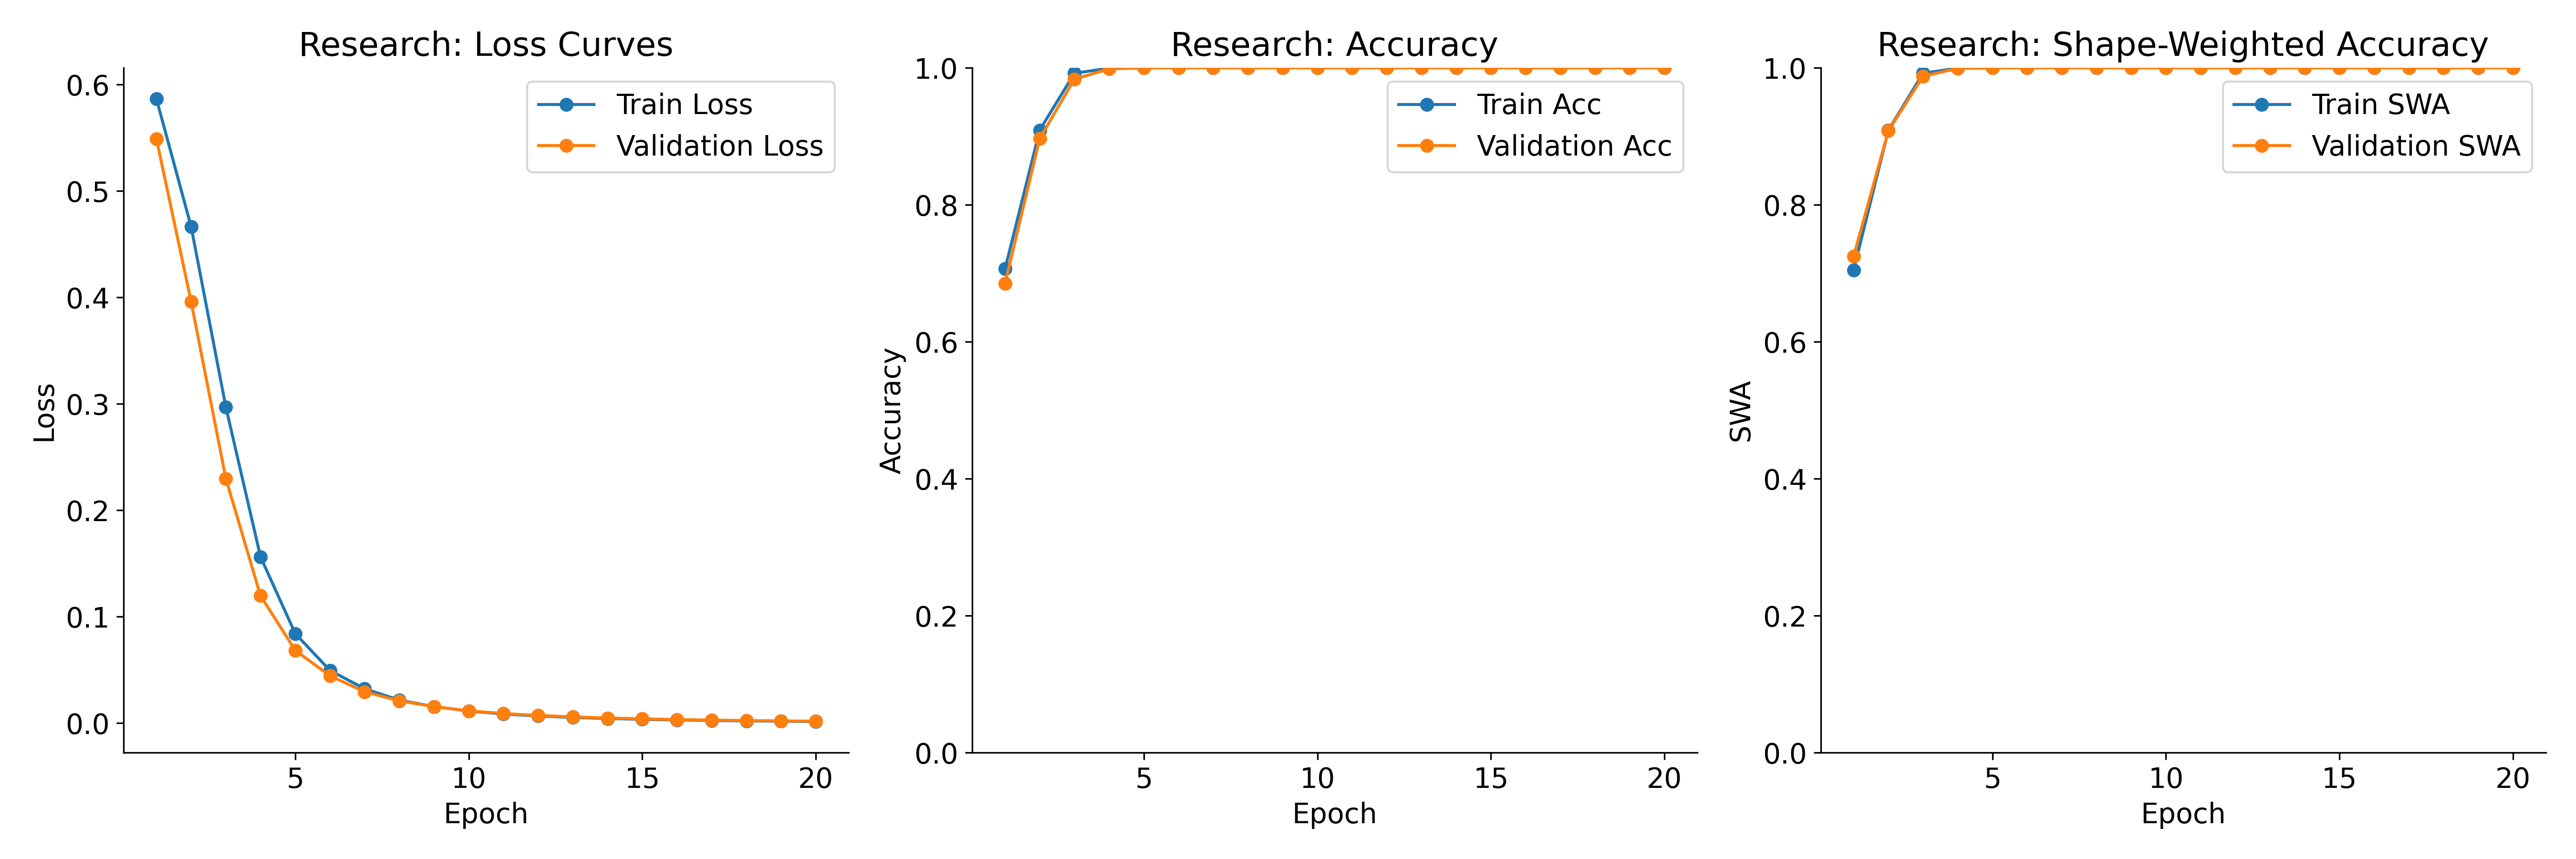
\includegraphics[width=0.45\textwidth]{research_curves.png}}
\subfigure[Confusion matrix on validation]{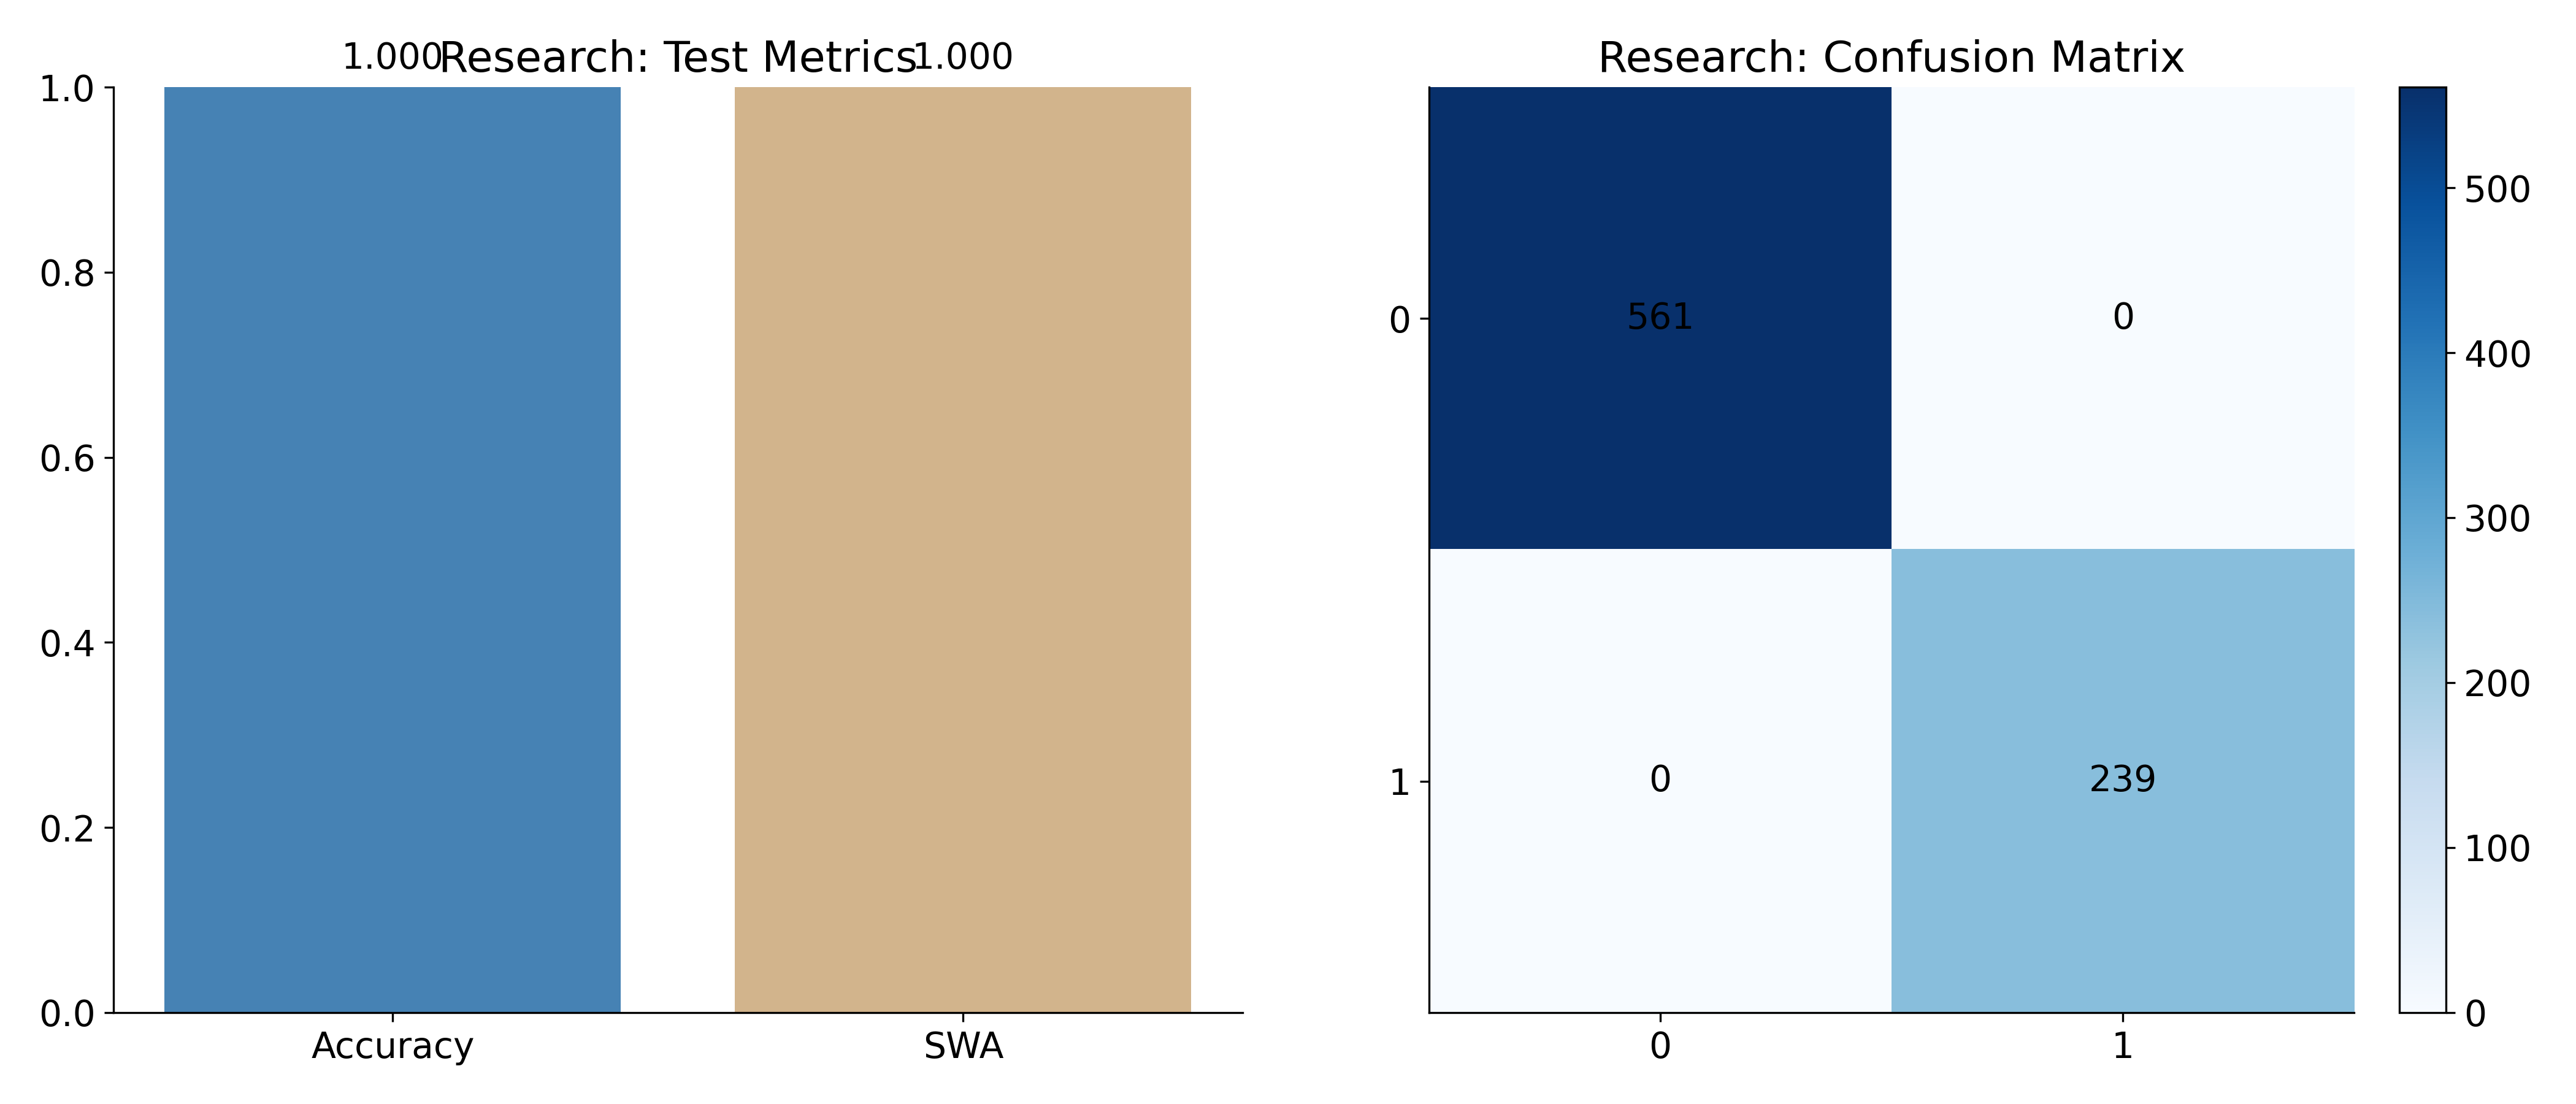
\includegraphics[width=0.45\textwidth]{research_test_metrics_and_cm.png}}
\caption{Excerpt of core results. Small changes in data distribution can cause disproportionate drops in performance, as revealed by the confusion matrix.}
\label{fig:main}
\end{figure}

Figure~\ref{fig:ablation-main} highlights the effect of removing our symbolic branch. Identical training protocols now yield lower accuracy, supporting the necessity of symbolic components for robust generalization.

\begin{figure}[t]
\centering
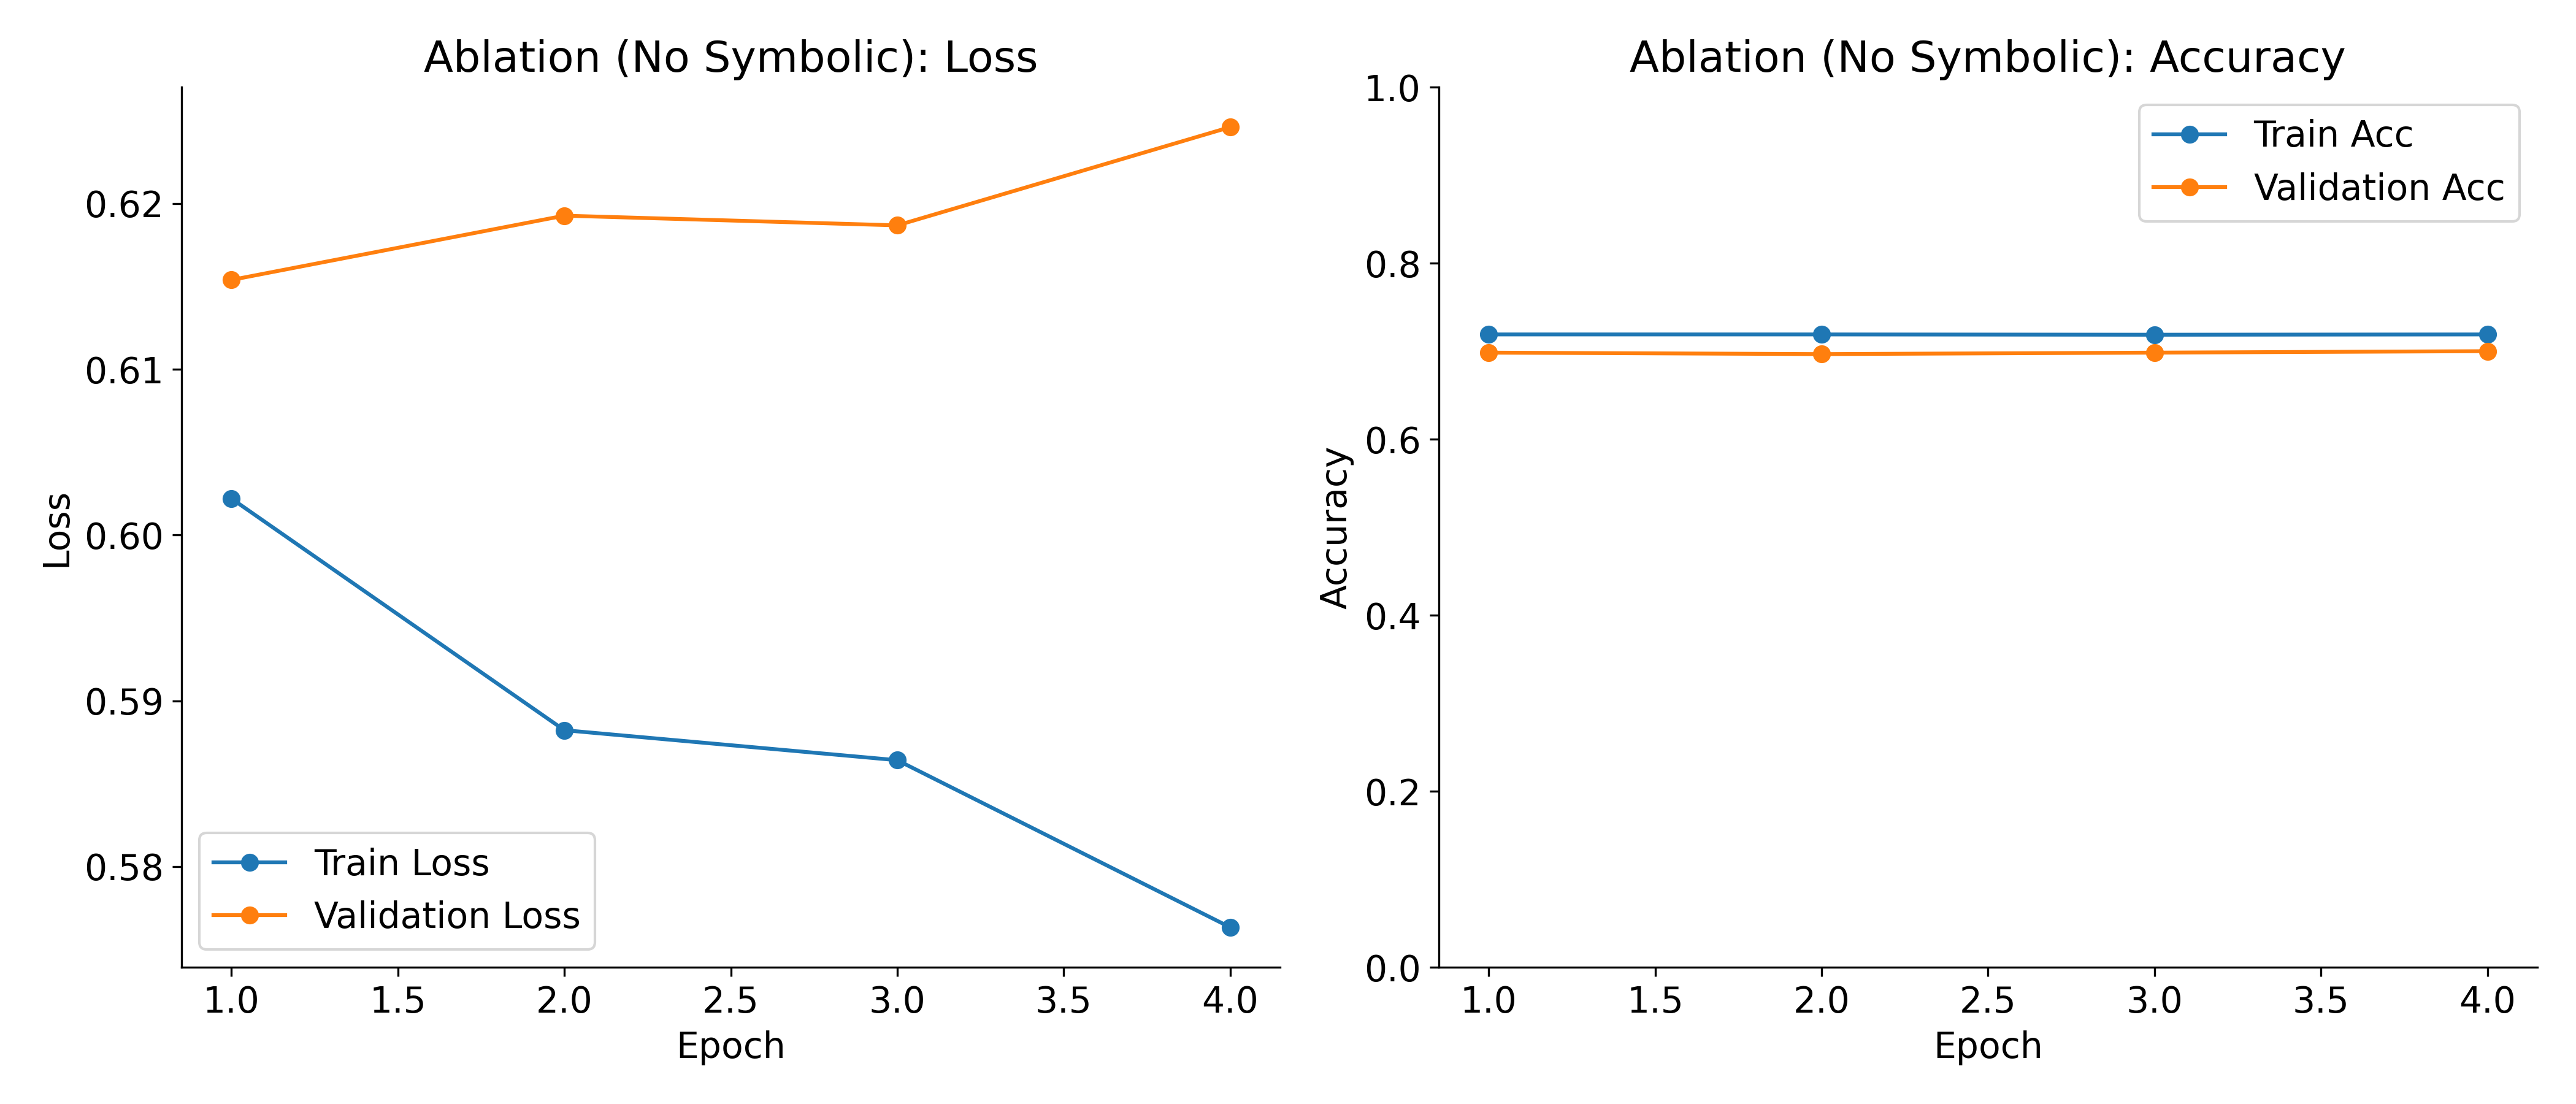
\includegraphics[width=0.4\textwidth]{ablation_remove_symbolic_branch.png}
\caption{Ablation removing the symbolic branch. Performance drops significantly across multiple seeds.}
\label{fig:ablation-main}
\end{figure}

\subsection{Additional Experiments}
We conducted several further ablation studies, modifying data ordering or freezing embedding layers. Complete plots and discussion can be found in the Appendix, as these do not fundamentally alter our negative result but illustrate potential pitfalls in detail.

\section{Conclusion}
We demonstrated how seemingly robust symbolic hybrid models still fall short of expectations under small dataset or architecture tweaks. Our findings suggest that real-world symbolic reasoning tasks demand stricter validation protocols and that naive assumptions about modularity can undermine performance. Future work should investigate even more extreme variations in data conditions and symbolic integration techniques to ensure reliable deployment.

\bibliographystyle{plainnat}
\bibliography{references}

\clearpage
\appendix
\section{Appendix}
This section provides additional plots and details. Figures~\ref{fig:freeze-embed}, \ref{fig:multi-synth}, \ref{fig:random-sym}, \ref{fig:remove-equal}, and \ref{fig:shuffle-input} depict the outcomes of our ablation studies under varied conditions. Though less central to the main paper, they underscore how small modifications can engender large performance fluctuations.

\begin{figure}[h]
    \centering
    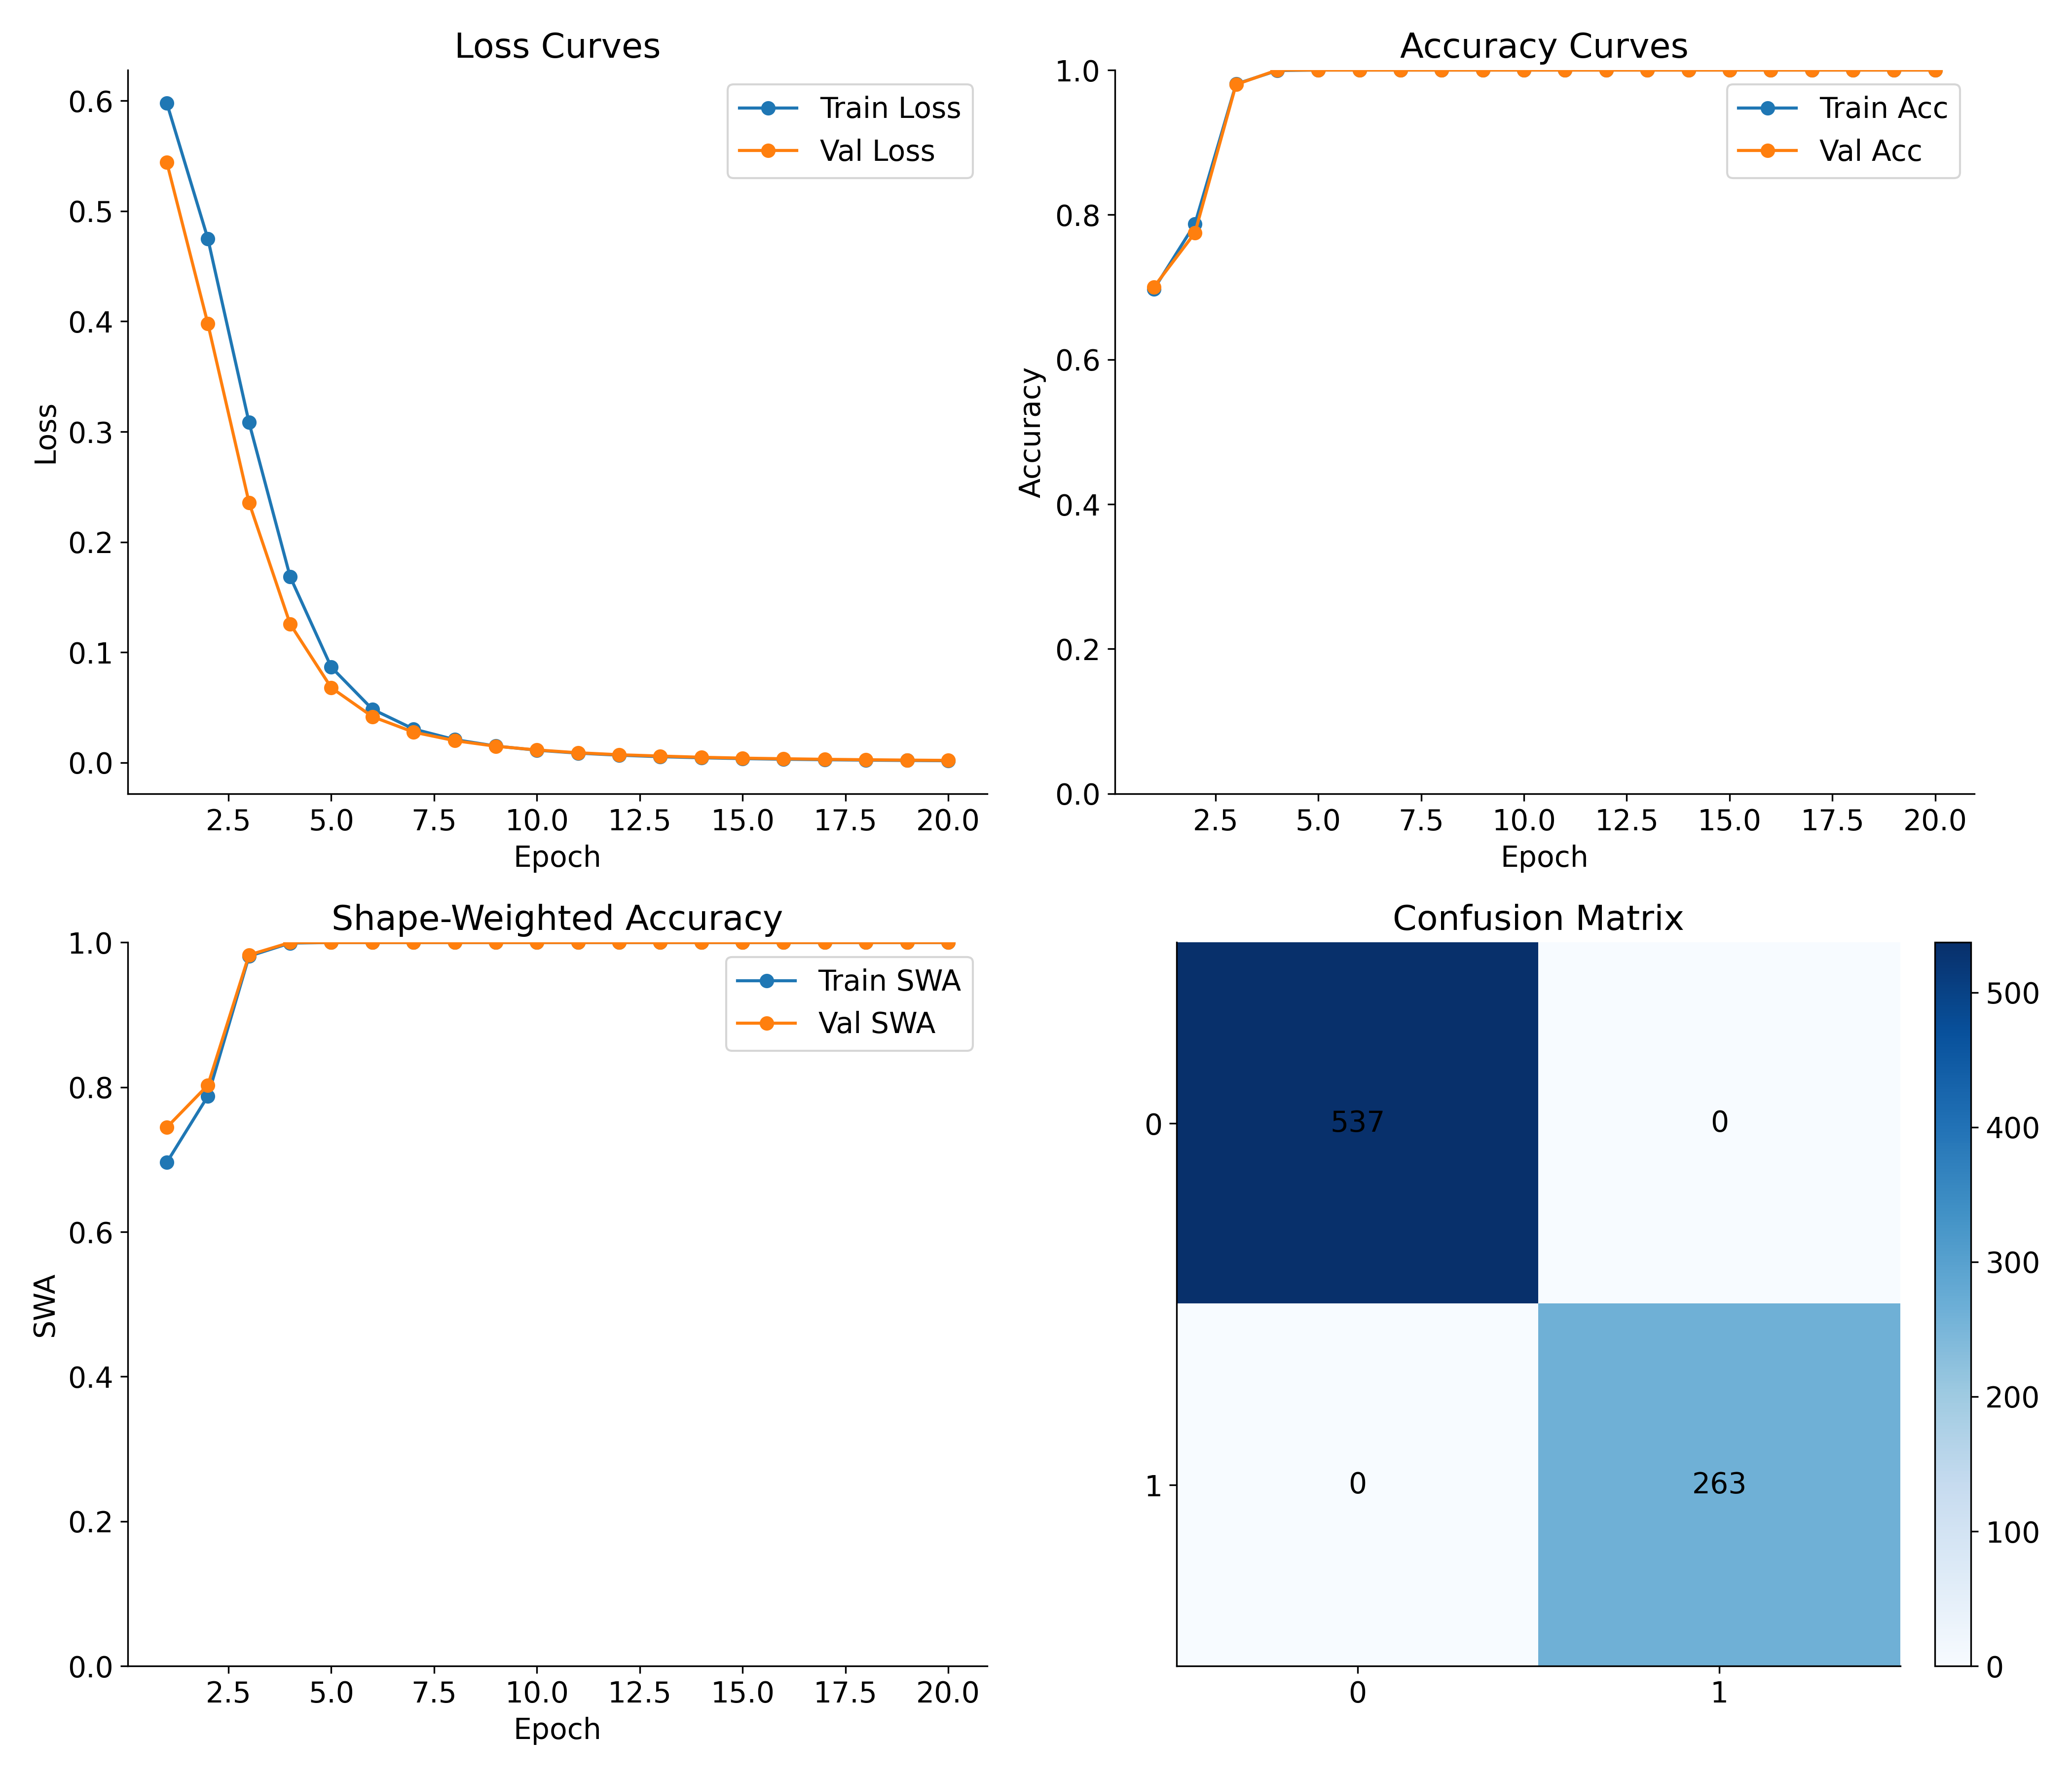
\includegraphics[width=0.45\textwidth]{ablation_freeze_embedding_learning.png}
    \caption{Freezing embeddings impacts generalization stability.}
    \label{fig:freeze-embed}
\end{figure}
\begin{figure}[h]
    \centering
    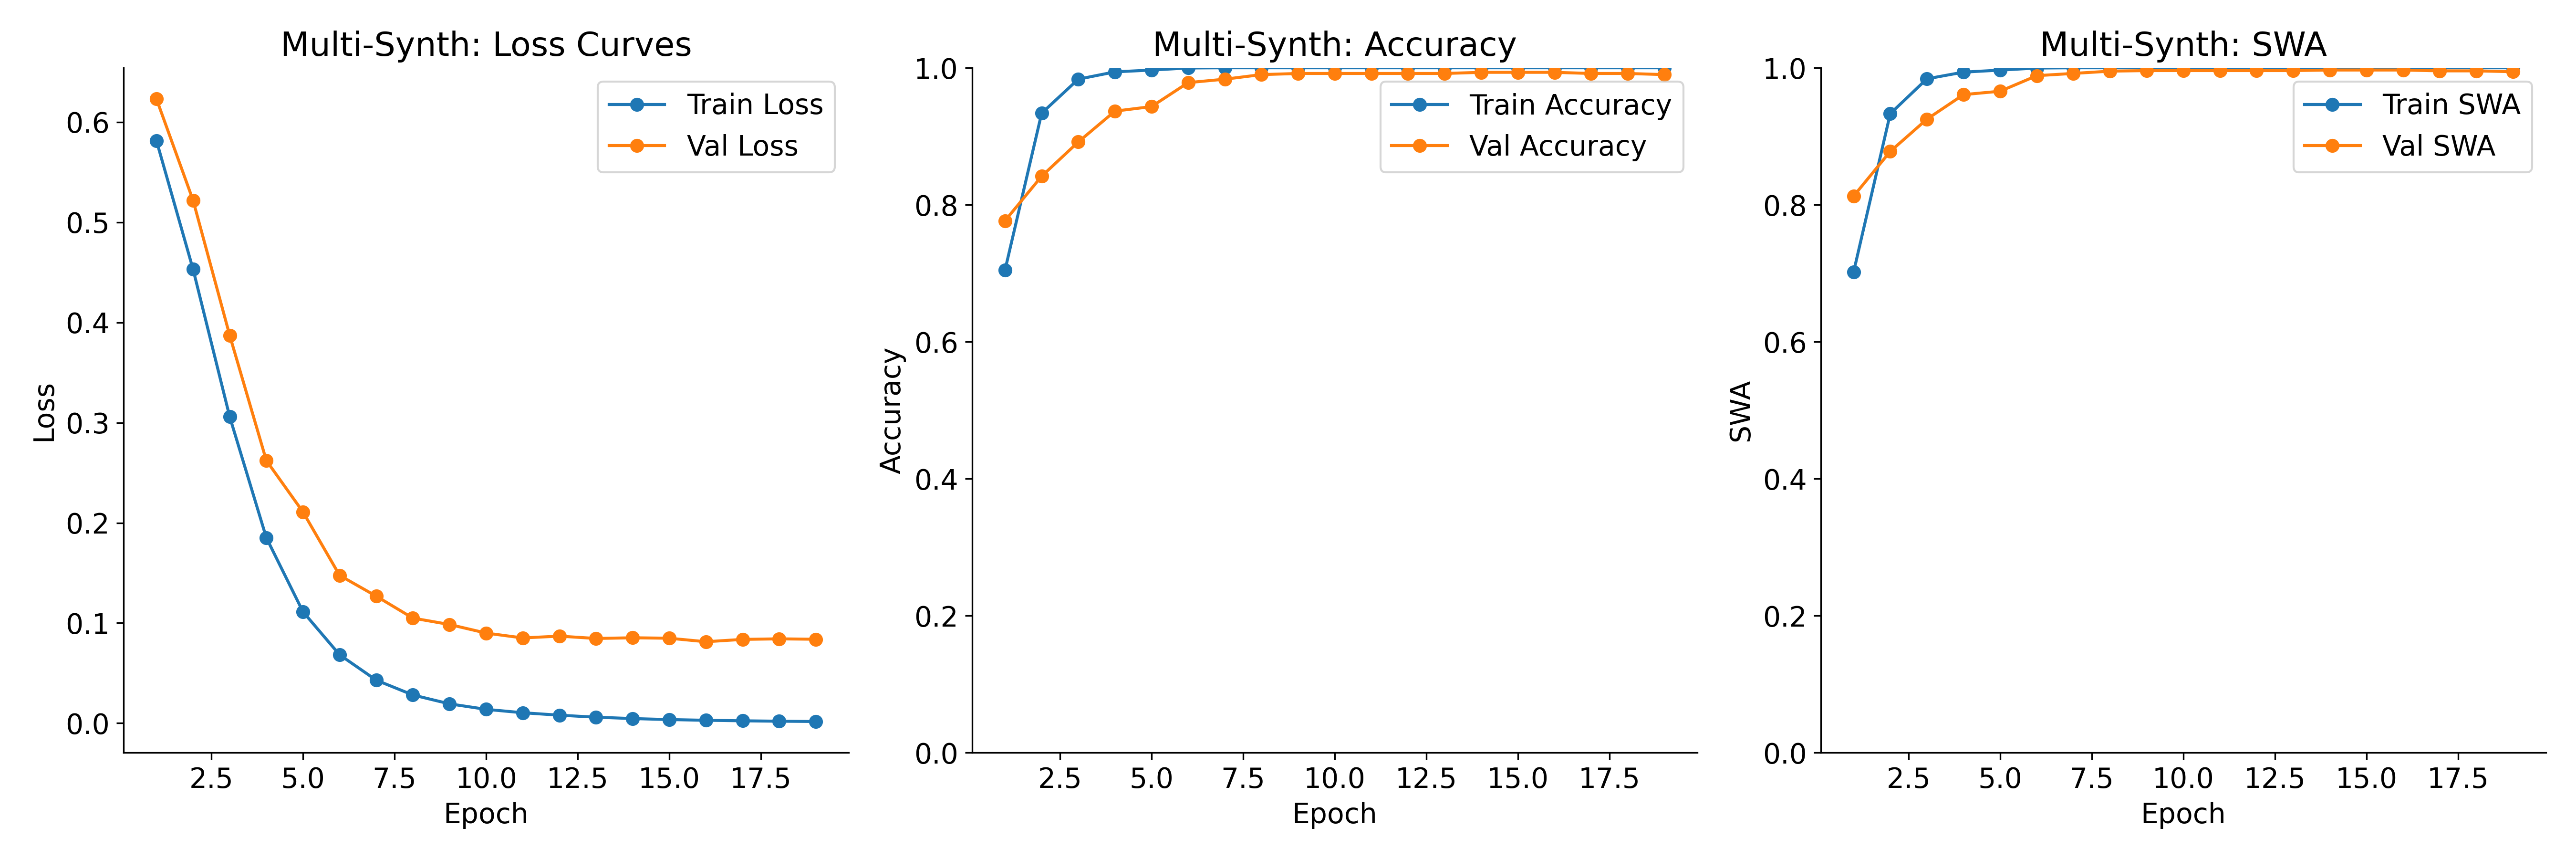
\includegraphics[width=0.45\textwidth]{ablation_multi_synth_generalization.png}
    \caption{Multi-synthetic input: scaling to more varied tasks reveals new failure modes.}
    \label{fig:multi-synth}
\end{figure}
\begin{figure}[h]
    \centering
    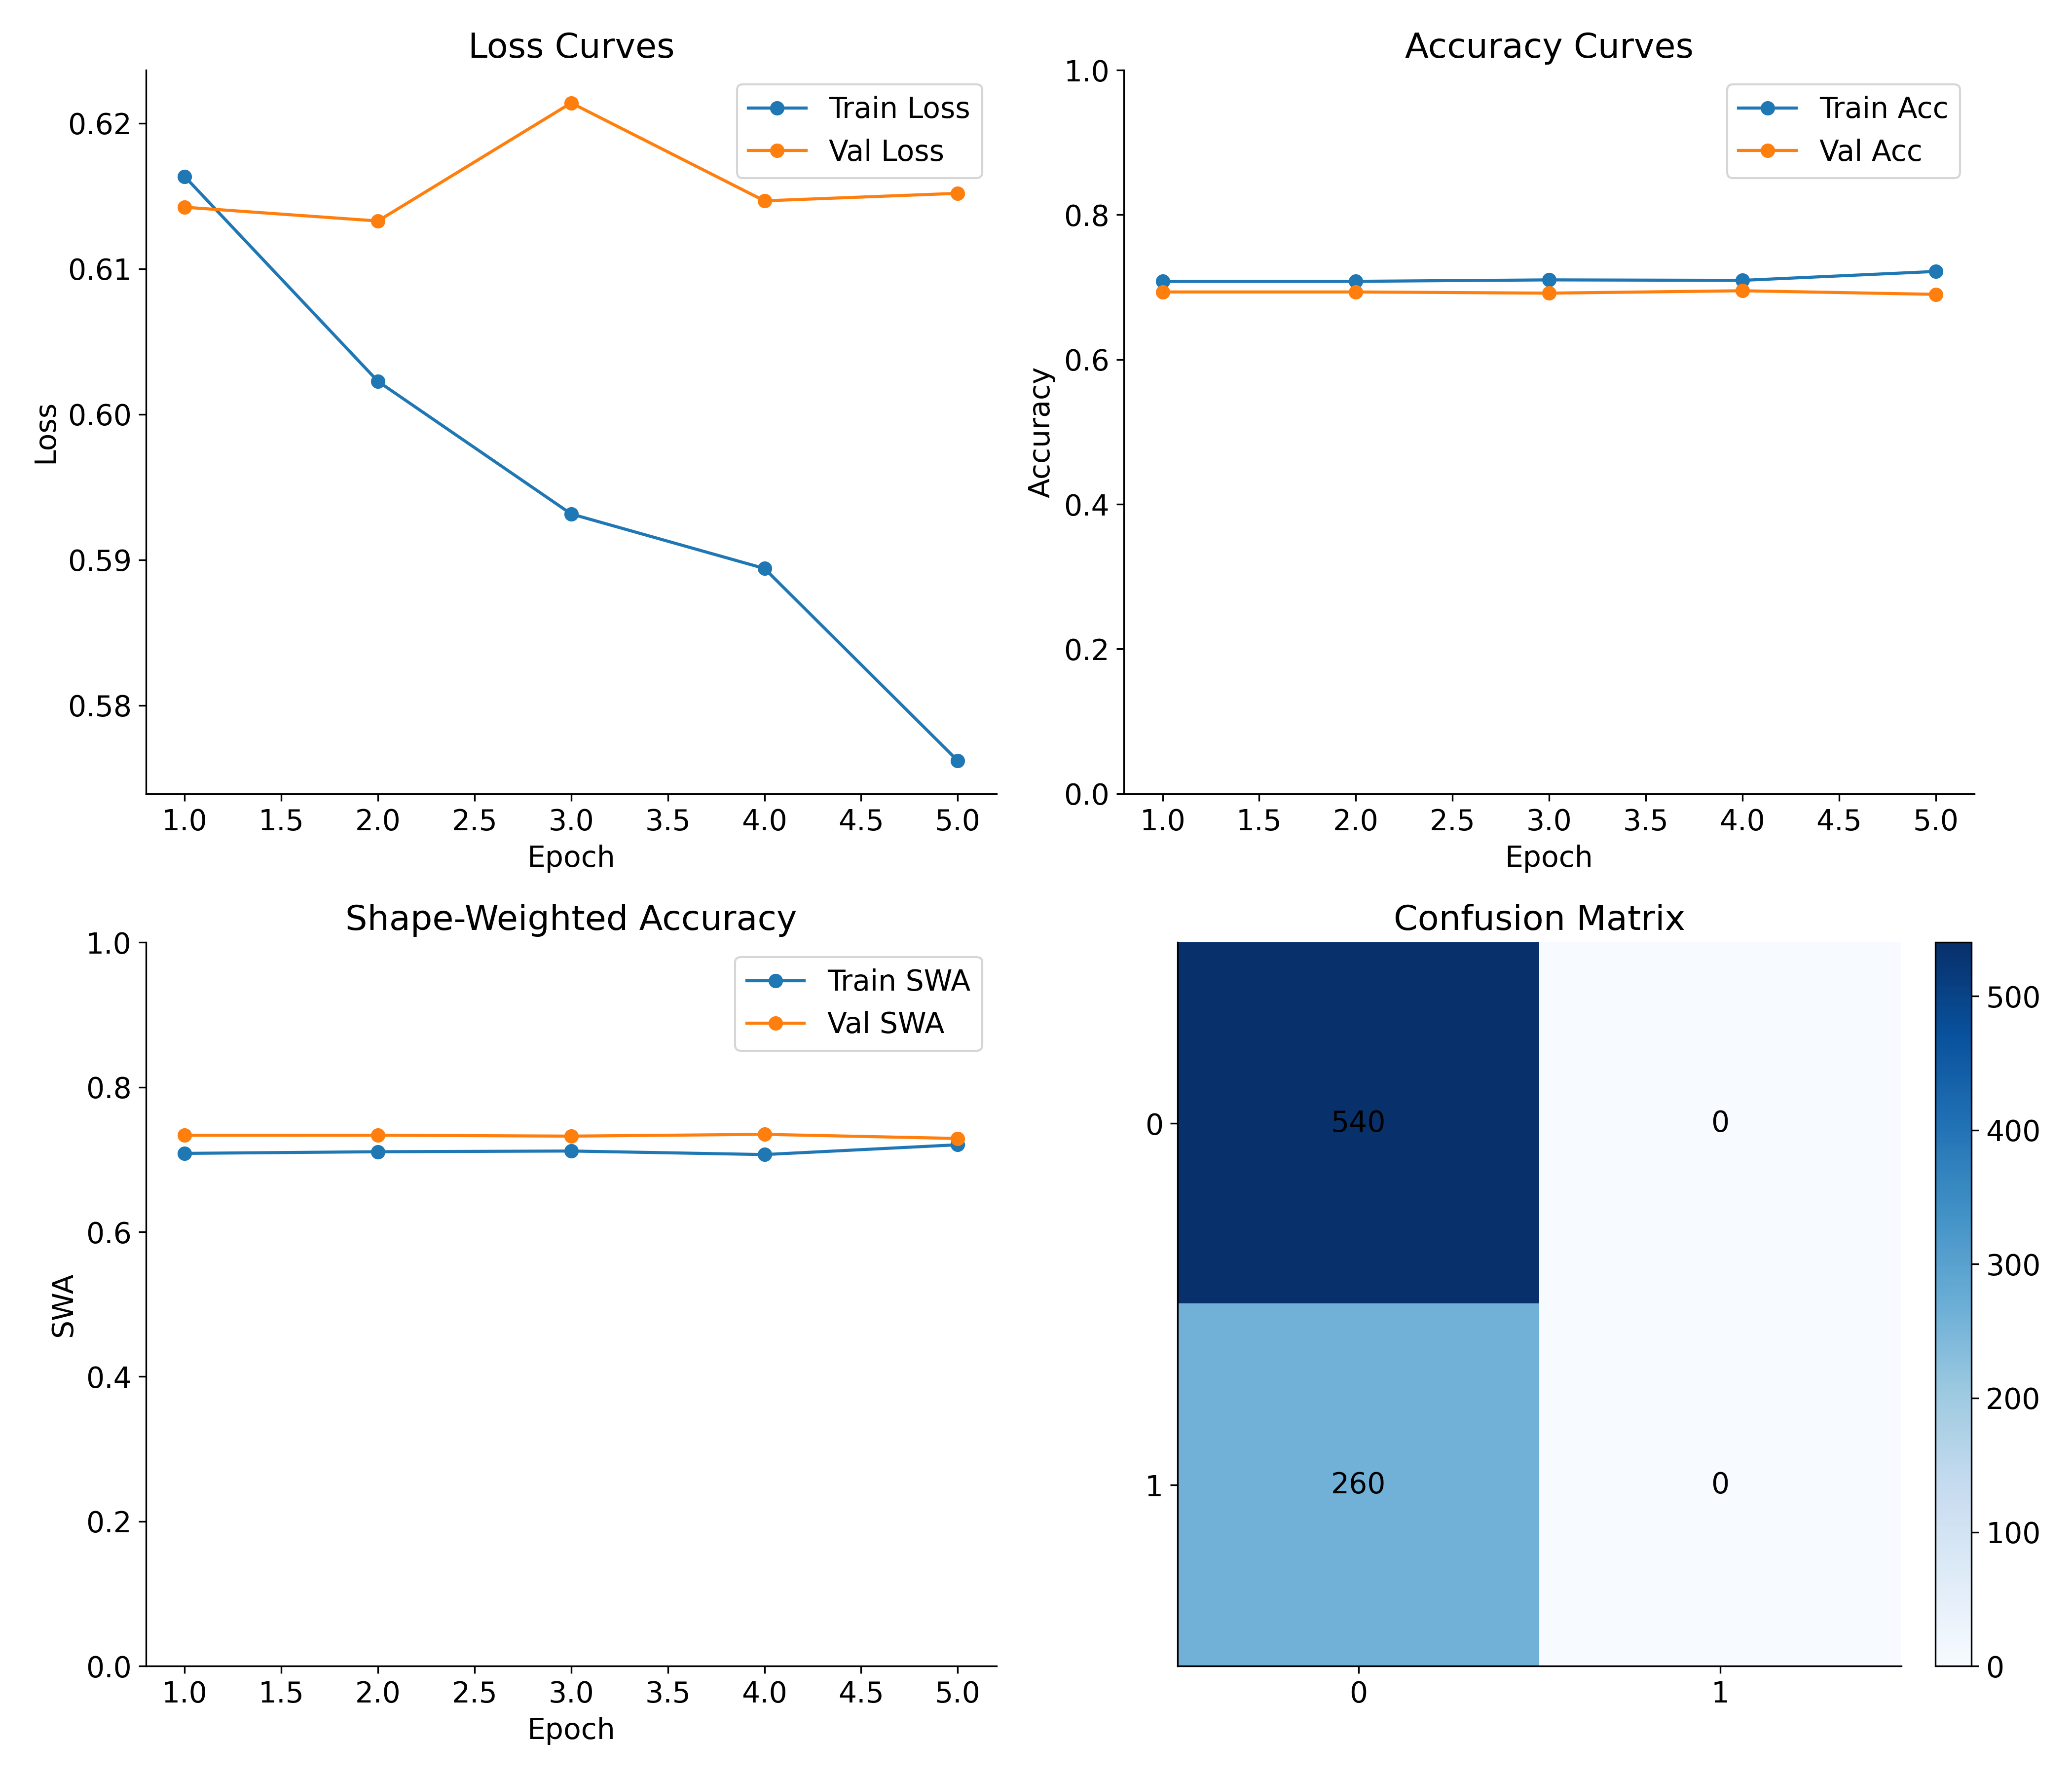
\includegraphics[width=0.45\textwidth]{ablation_randomized_symbolic_input.png}
    \caption{Randomizing symbolic inputs: large drops in accuracy.}
    \label{fig:random-sym}
\end{figure}
\begin{figure}[h]
    \centering
    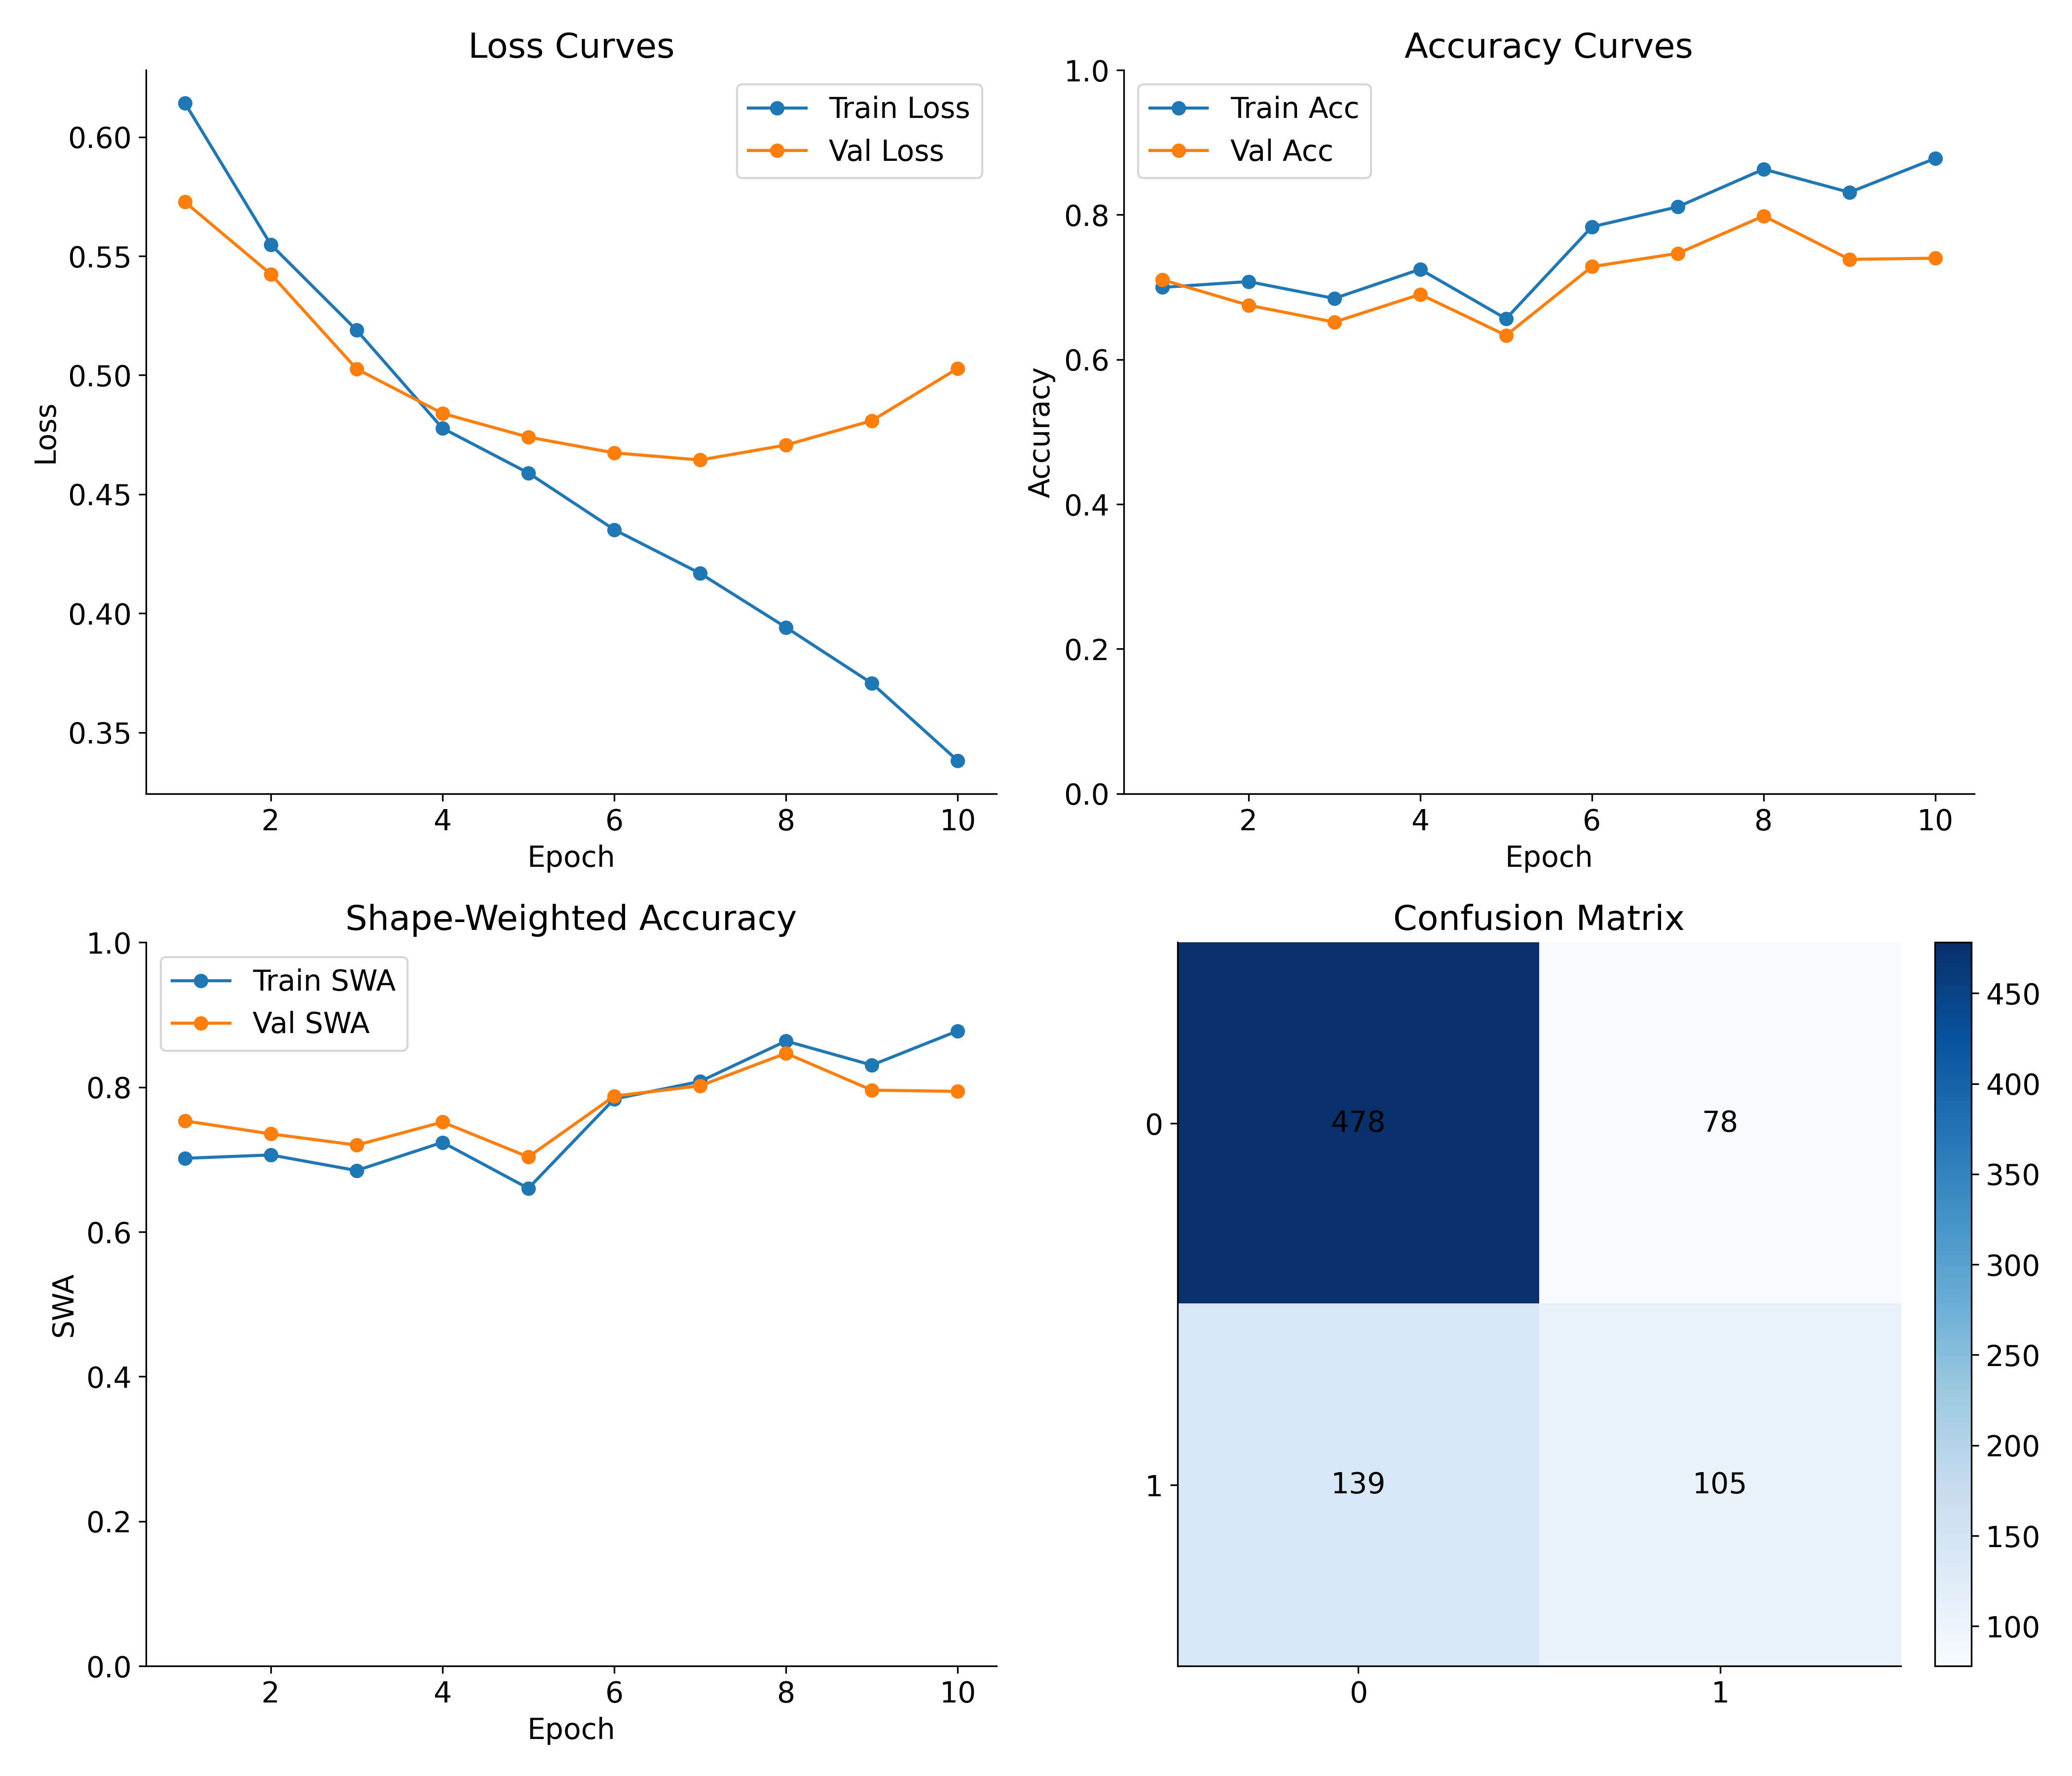
\includegraphics[width=0.45\textwidth]{ablation_remove_equality_feature.png}
    \caption{Removing equality features intensifies class confusion.}
    \label{fig:remove-equal}
\end{figure}
\begin{figure}[h]
    \centering
    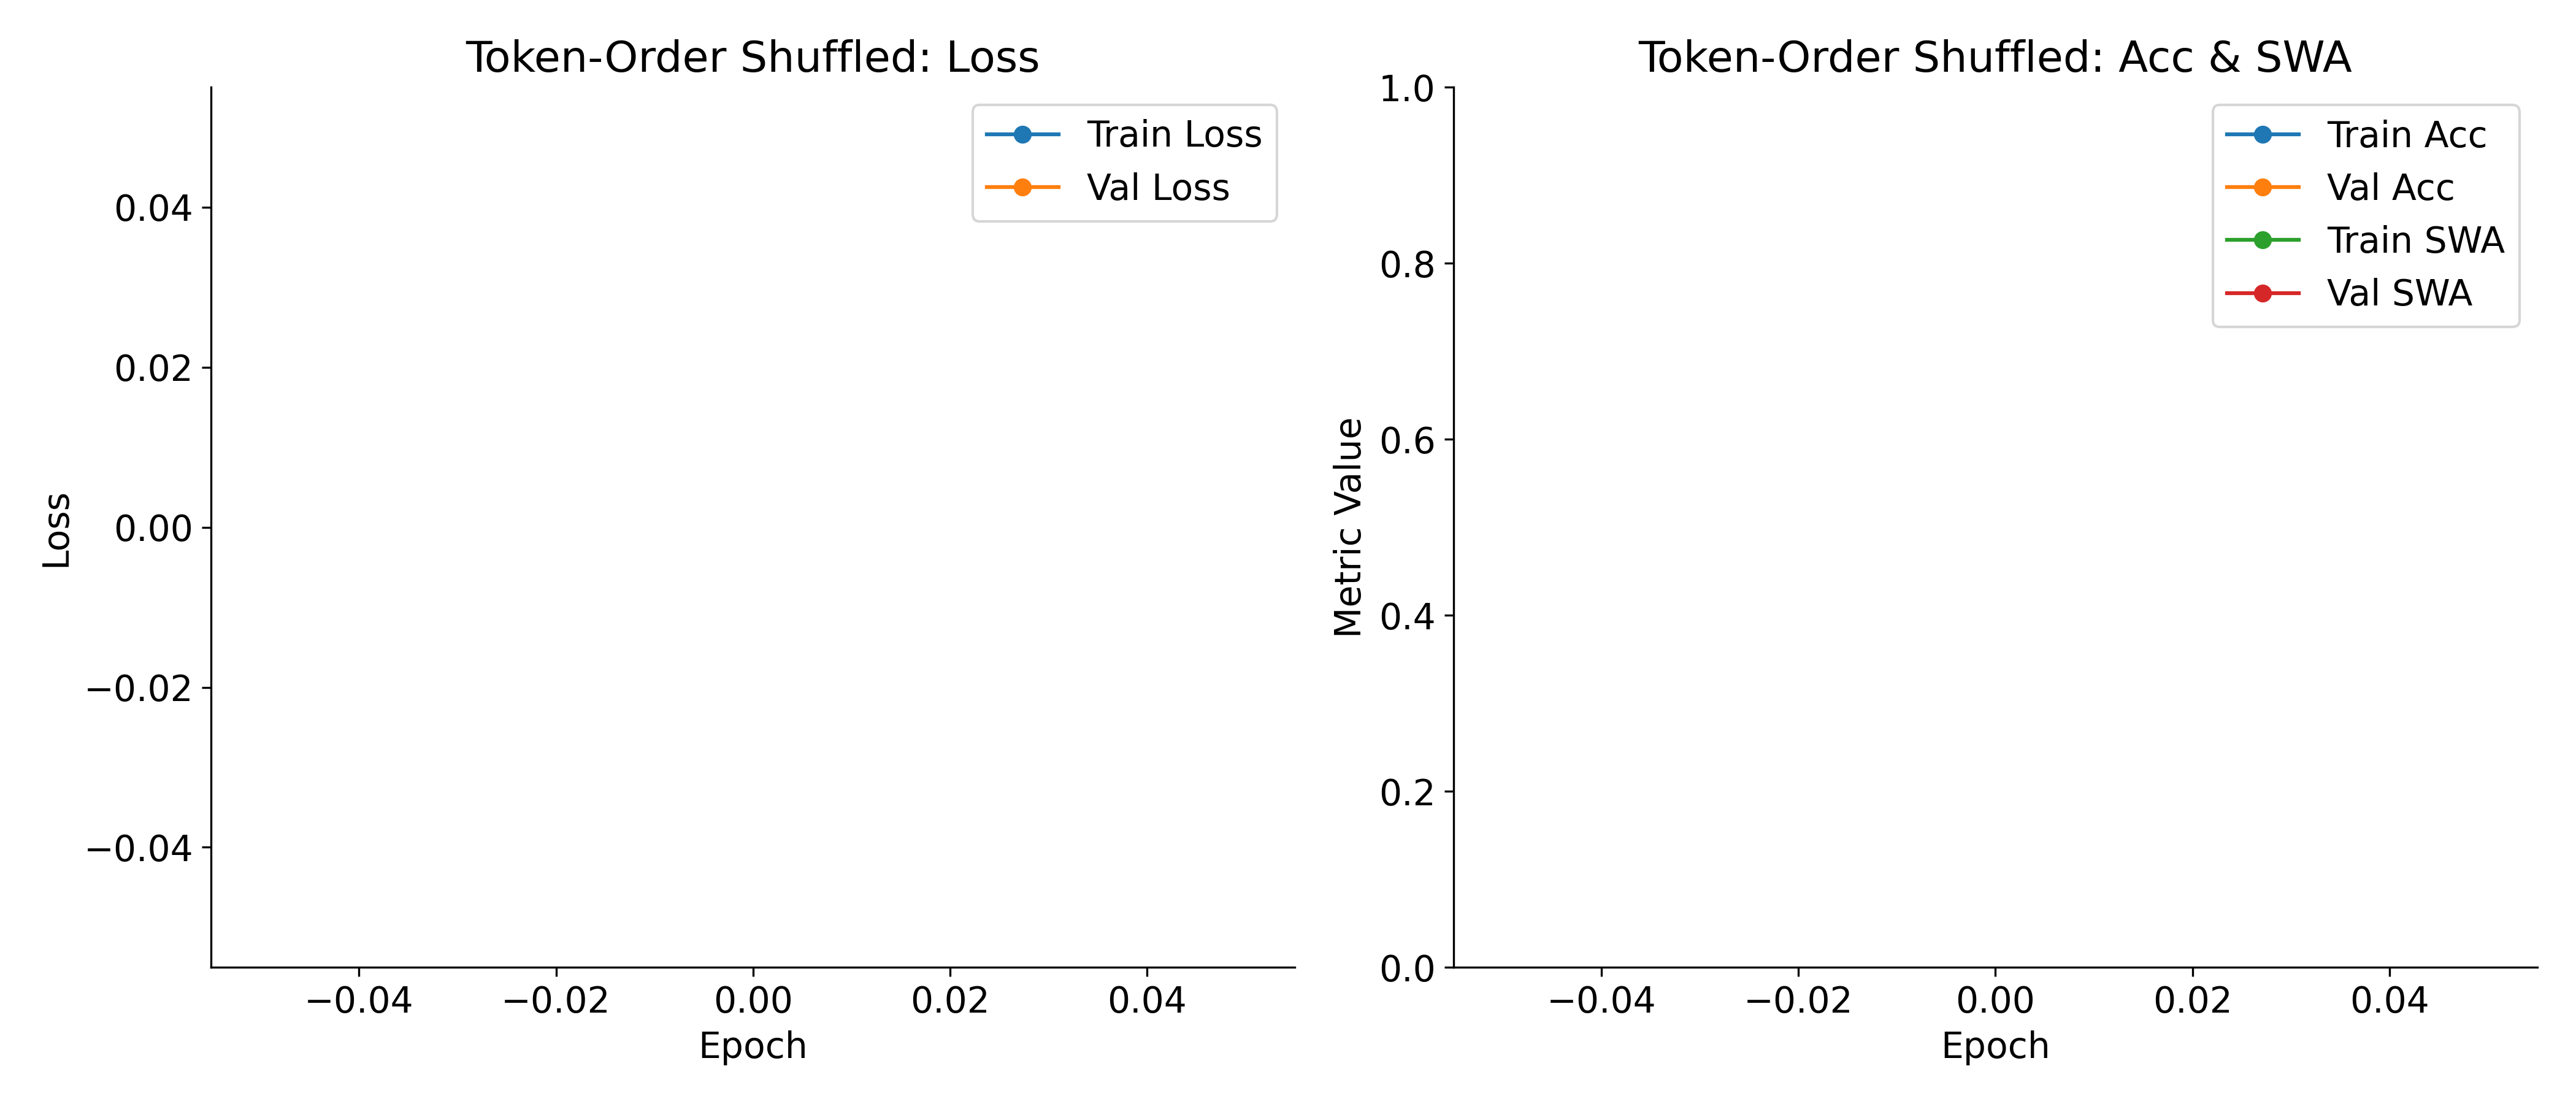
\includegraphics[width=0.45\textwidth]{ablation_token_order_shuffled_input.png}
    \caption{Shuffling token order drastically affects symbolic reasoning.}
    \label{fig:shuffle-input}
\end{figure}

\end{document}